\chapter[Mixing Properties of Individual Enrichment Sources]{Mixing Properties of Individual Enrichment Sources\label{ch:chapter4}}
\begingroup
\let\thefootnote\relax\footnotetext{This section contains unpublished work-in-progress}
\endgroup

%
% Copy paste paper here, without abstract or keywords
%

\newcommand{\runone}{I\_}
\newcommand{\runonenu}{I}
\newcommand{\runtwo}{II\_}
\newcommand{\runtwonu}{II}

\section{Introduction}

The elemental abundances of a galaxy over time are sensitive to the nuclear physics and stellar astrophysics that determines which stars make what elements and when. The stellar abundance patters within a given galaxy also depend on the details of how those metals are released into the ISM through various forms of stellar feedback, and the hydrodynamic interactions that ultimately mix those elements into the ISM or eject them from the galaxy in galactic winds. Stellar abundance patterns in old, metal poor systems are the result of enrichment from substantially fewer sources than younger, more metal rich stellar populations. Because of this, studying abundance patterns in these environments allows us to place constraints on the yields of individual enrichment events and the nucleosynthetic sites of each element. The lowest mass dwarf galaxies in the Local Group, UFDs, offer some of the best constraints on these processes. These environments can potentially be used to trace and constrain enrichment from the first stars \citep[e.g.][]{FrebelBromm2012,Ji2015,Ritter2015,Jeon2017,Hartwig2018}. and have been used to place constraints on the variety of possible astrophysical sources of r-process enrichment \citep[e.g.][]{Ji2016a,Ji2016b,Ji2018a,Ji2019,Tsujimoto2017,Duggan2018,Nagasawa2018,Ojima2018}. It is likely that chemical enrichment in more massive, metal rich systems with ongoing star formation like the Milky Way is much more uniform, averaging over the variety of complex hydrodynamics and feedback-driven turbulence interactions that may be driving much of the significant variance in stellar abundances seen at low metallicity. Stochasticity, which has been shown to be important for setting the width of stellar abundance patterns low metallicity environments of the Milky Way \citep[e.g.][]{Cescutti2008,Cescutti2014}, plays an even greater role in the evolution of these low mass dwarf galaxies \citep{Applebaum2018}. Indeed the increase in scatter in the stellar abundance patters of low mass dwarf galaxies and UFDs has been attributed to inhomogeneous mixing and stochastic effects \citep[e.g.][]{Norris2010a,Simon2015,Mashonkina2017,Suda2017}. This complicates the interpretation of abundance patters in these galaxies, particularly for constraining individual enrichment events.

% Maybe cite Norris2010a, Simon2015, Nissen1994 for abundance spreads in UFDs?

Recent cosmological zoom simulations have attained sufficient resolution to follow the evolution of individual UFDs (or their progenitors at high redshift) and can investigate their chemical properties \citep{Jeon2017,Corlies2018,Escala2018,Christensen2018}. Additional works have conducted more direct investigations into what drives the enrichment process for individual sources using both hydrodynamics simulations \citep{PanScannapiecoScalo2013,Ritter2015,Safarzadeh2017,Hirai2015,Hirai2017,Emerick2018b,HaynesKobayashi2019} and semi-analytic models \citep{Beniamini2018,KrumholzTing2018}. In \cite{Emerick2018b} we demonstrate that elements released through AGB winds have both wider abundance distributions in the ISM and lower ejection fractions from the galaxy than elements released in supernovae. It is becoming increasingly clear that enrichment is quite inhomogeneous in low mass dwarf galaxies (refs?), and also that the behavior of metals from any one enrichment event depends on a significant number of complex interactions. In spite of this progress, there is still substantial work to be done in understanding the physical processes that drive both evolution of both the mean and width of stellar abundances in low-mass dwarf galaxies.

In this Chapter we utilize the simulations analyzed in prior chapters to conduct a controlled set of ``mixing experiments'' whereby we restart each simulation with enrichment events placed by-hand in order to more directly investigate the evolution of metals from an individual event. While elemental yields were tracked for each star in our simulation, we lacked the necessary Lagrangian information about the metals once they were released into the ISM to be able to trace the evolution of single enrichment events. We investigate primarily how the feedback ejection energy of individual sources ($E_{\rm ej}$) and global star formation rate at the time of enrichment affects how metals are ejected from the galaxy in galactic winds and metal mixing in the ISM. In Section~\ref{ch4:sec:methods} we briefly outline our methods and discuss the setup of these mixing experiments. In Section~\ref{ch4:sec:results} we discuss the results of these experiments and the role of $E_{\rm ej}$, global SFR, radial position of the enrichment event, and local ISM density around each enrichment sources affects the evolution of its metals, and discuss and conclude in Section~\ref{ch4:sec:discussion conclusion}.


\section{Methods}
\label{ch4:sec:methods}
We refer the reader to the previous chapters for more detailed descriptions of our numerical methods and feedback models. The mixing experiments discussed below are conducted in restarted versions of the same low-mass, isolated galaxy simulations used throughout this work.


%We refer the reader to Paper I for a detailed description of our numerical methods and feedback models. We briefly summarize the relevant details here.

% Summarize details here for the paper, but I'm not sure if its needed for the thesis chapter.

\subsection{Mixing Experiment Setup}
\label{ch4:sec:experiment}
We restart our fiducial, full-physics simulation at two different times, 180 Myr, and 360 Myr, labeled as runs \runonenu~ and \runtwonu~ respectively. These correspond to two different times in the galaxy's SFR evolution, testing how much variance is expected in the metal mixing and ejection with the star formation rate. \runonenu~ occurs during the lull in star formation following the initial SFR peak, and \runtwonu~ occurs in an extended period of little to no ongoing star formation. We attempted to to evolve each simulation for 150 Myr, but due to computational constrains this was not always possible.\footnote{We began runs during the peak of star formation ($\sim 100$~Myr), but the computational cost increases substantially during this time. These runs were abandoned.}

% I occurs in the last $\sim$ 20 Myr of the initial burst of star formation,

At the beginning of each restart, we place by-hand one or more enrichment events at assigned positions throughout the galaxy, with thermal injection energies ($E_{\rm ej}$), masses ($m_{\rm ej}$), and metal fractions ($Z_{\rm ej}$). We note that the injection masses, particularly the metal fractions, are somewhat arbitrary as they are likely dynamically insignificant relative to the ambient ISM mass in which they occur. The important parameter here is $E_{\rm ej}$, which we vary to sample the range of ejection energies associated with significant sources of chemical enrichment, including AGB winds ($10^{46}$~erg)\footnote{Assuming full thermalization of the total mechanical energy output of an AGB wind.}, NS-NS mergers ($10^{49} - 10^{50}$~erg), supernovae (10$^{51}$~erg), and exotic enrichment sources, such as hypernovae, that can reach much higher energies (10$^{52}$~erg). Each run contains only sources from a single event type, as indicated in the run-name by the log of the injection energy in ergs. For example, the run beginning at 180~Myr with AGB-like events is labeled ``\runone E46". The metal enrichment from each source is tracked and evolved with a unique passive scalar tied to the individual source and separate from any additional chemical enrichment that may occur within the galaxy over time.

Each run contains multiple events spread over the galaxy to test how radial and azimuthal position in the galaxy affects mixing and ejection, but limited to ensure that the events do not overlap and influence each other dynamically. For the low-energy events, we are able to run 19 events per restart, while the $10^{49}-10^{51}$~erg runs contain 7 events, and the 10$^{52}$~erg runs only contain a single event.

Most of this analysis refers to these average behavior of the metals from these enrichment events over time as a way to gain a general appreciation for how $E_{\rm ej}$ and galactic properties affect the evolution of metals. However, we do note that this is not fair statistically, as the higher energy runs are undersampled.

%We discuss how radial and azimuthal position affects the evolution in


\section{Results}
\label{ch4:sec:results}
Perhaps the three most important parameters to quantify for each enrichment event are: 1) what fraction of released metals are immediately available for star formation, 2) what fraction of metals are carried out of the galaxy in outflows, and 3) how and over what timescale do metals cool from hot phases into star forming gas. We discuss each of these points in Section~\ref{ch4:sec:ISM CGM}. In Section~\ref{ch4:sec:spreads} we go further and address the relative homogeneity of the metals retained by the ISM for each enrichment source.

\subsection{Enrichment of the ISM and CGM}
\label{ch4:sec:ISM CGM}

\begin{figure*}
\centering
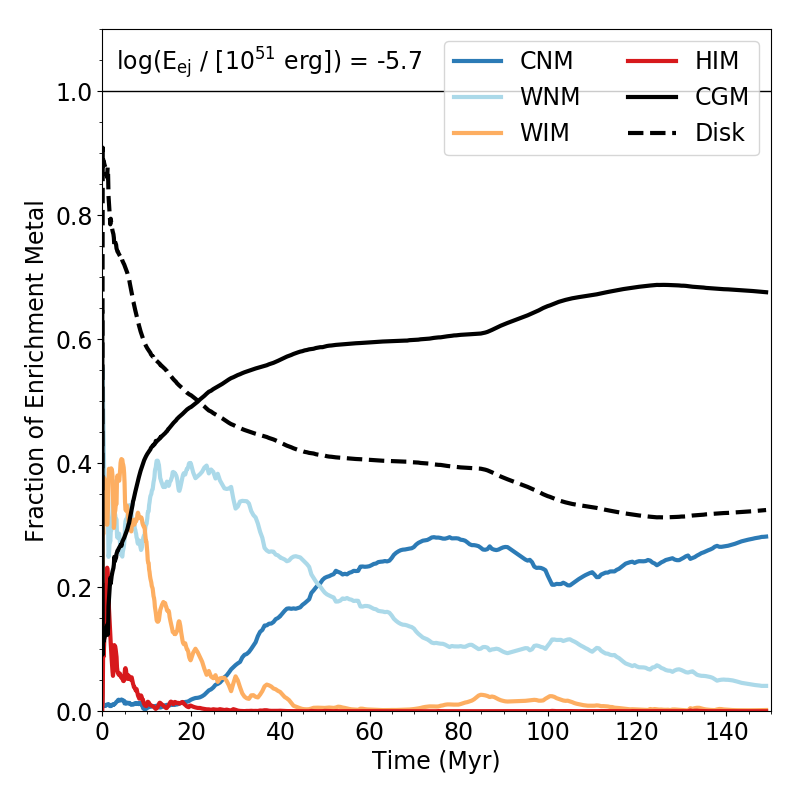
\includegraphics[width=0.45\linewidth]{figures/ch4/AGB1_enrichment_evolution_average_CGM}
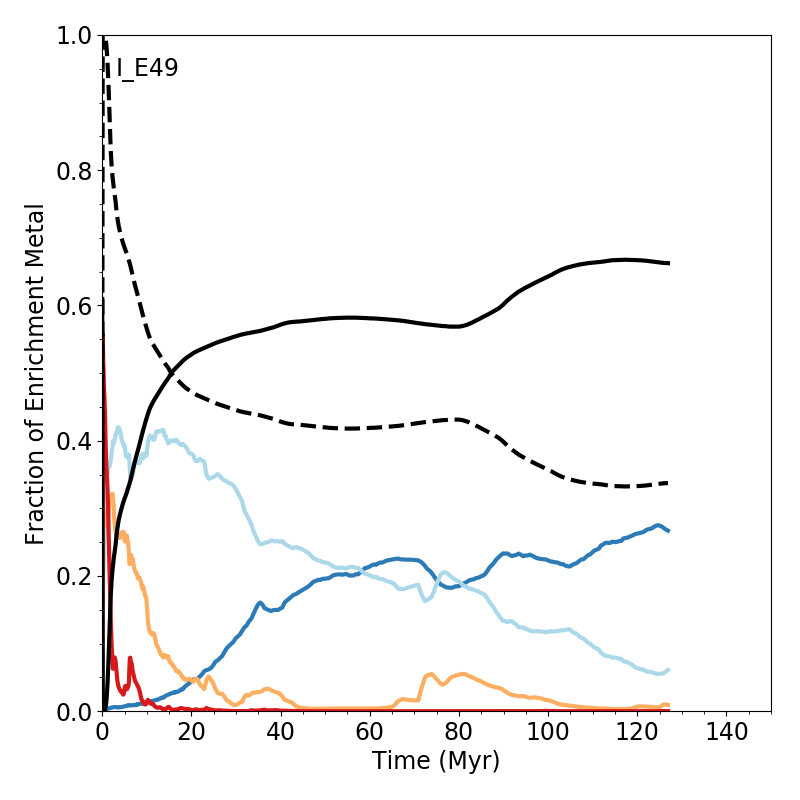
\includegraphics[width=0.45\linewidth]{figures/ch4/NSNS1_enrichment_evolution_average_CGM} \\
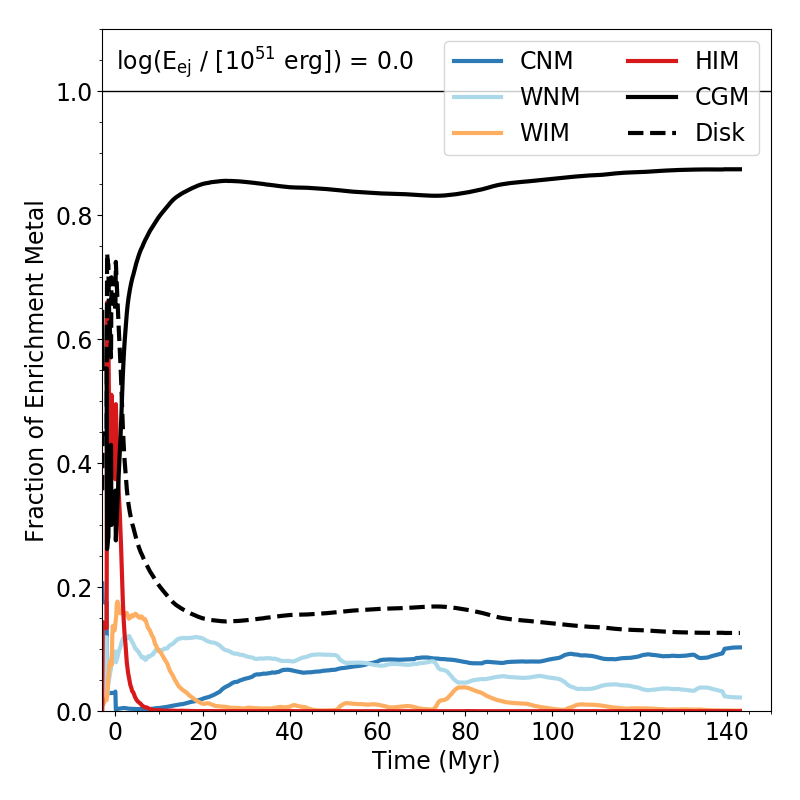
\includegraphics[width=0.45\linewidth]{figures/ch4/SNE1_enrichment_evolution_average_CGM}
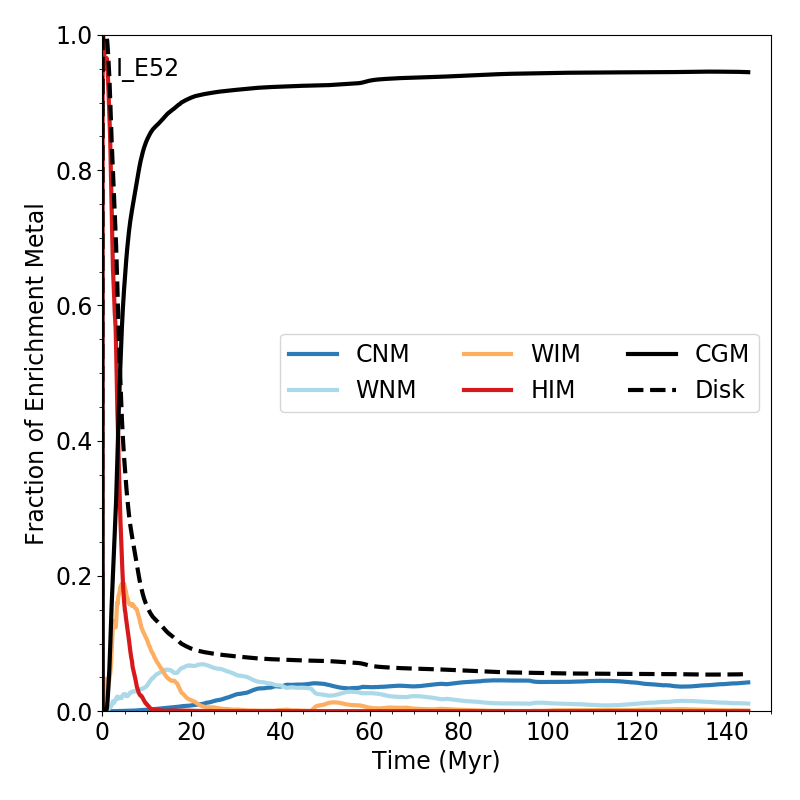
\includegraphics[width=0.45\linewidth]{figures/ch4/HNE1_enrichment_evolution_average_CGM}
\caption{Time evolution of the }
\label{ch4:fig:ISM_CGM}
\end{figure*}

We summarize the source-averaged results for all enrichment events in runs \runone E46, \runone E49, \runone E50, \runone E51, and \runone E52 in Figure~\ref{ch4:fig:ISM_CGM} by showing the fraction of source metals contained within each phase of the ISM (colored lines, which sum to the black dashed line), and the CGM (black, solid). These plots show a clear, immediate trend across $E_{\rm ej}$ for all lines in the figure, but the differences are most striking for the ISM (black, solid), CGM (black, dashed) lines. In Chapter~\ref{ch:chapter3}
% \citep{Emerick2019}
we demonstrated that there was a significant difference in metal ejection fraction, $f_{\rm ej}$, for metals from AGB sources as compared to metals released in SNe. Here, we confirm that this is driven predominantly by differences in the energy of the events, and not necessarily when or where they occur in the ISM. The clear trend in Figure~\ref{ch4:fig:ISM_CGM} shows that events with higher $E_{\rm ej}$ are much more readily ejected from the disk of the galaxy, while events with lower $E_{\rm ej}$ couple poorly to the same galactic outflows.
%\textit{statement on how immediate enrichment is after events}
% By 10~Myr after the enrichment events,
The high-energy events rapidly converge on a peak $f_{\rm ej}$ within about 20~Myr of the event, with only a gradual increase towards the end of the 150~Myr as the metals in the ISM are swept up in additional outflows. The lower energy events evolve more gradually. The lowest energy event, corresponding to AGB winds, reaches $f_{\rm ej}$ ~ 0.68, which increases to 0.87 for the 10$^{51}$~erg events, and 0.95 for the 10$^{52}$~erg event. To emphasize these differences, we plot each line separately in the left panel of Figure~\ref{ch4:fig:CGM_CNM}

This implies that, if one to were assume that all metals behaved the same and adopted an $f_{\rm ej}$ of $\sim$0.9 -- typical for the total metal ejection fraction in simulations that do not track individual enrichment channels \citep[e.g.][]{Muratov2017,Christensen2018}, and consistent with observations of the O abundance in Local Group dwarf galaxies \citep[e.g.][]{Kirby2011,McQuinn2015} -- one would underestimate the amount of AGB metals in the ISM by a factor of $\sim$ 3, and overestimate exotic, high-energy sources by a factor of $\sim$ 2. In each case, these are metals that cannot participate in the enrichment of future stellar populations and will make a significant difference on the output stellar abundances in chemical evolution models. We explore this impact in different works.

In all cases, the metals contained with the ISM are deposited predominately in the ionized phases of the ISM, the WIM or the HIM, with the relative fraction in each phase driven by the energy of the event. Metals in the ISM injected with $E_{\rm ej} > 10^{49}$~erg are initially located predominately in the HIM, roughly 1/2 for $E_{\rm ej} = 10^{49}$~erg and nearly all for $E_{\rm ej} > 10^{51}$~erg. The lowest energy events are initially in the WIM and WNM, tracing the two dominant volume-filling components of the ISM (see Chapter~\ref{ch:chapter1}), as these events do not have sufficient energy to generate the HIM by themselves.

Gas above the star formation threshold in our simulations is limited and short-lived due to the low gas surface densities and star formation rates in this galaxy and the efficiency of stellar feedback from newly formed stars. As a proxy, we examine the evolution of the CNM, out of which the star forming gas forms. In general, very few of these elements are available for immediate star formation in the CNM ($<< 1\%$, see Figure~\ref{ch4:fig:CGM_CNM}). However, we note that we may not have sufficient resolution to properly resolve the details of the initial mixing of individual enrichment events in the ISM. In addition, this value will be sensitive to whether or not a given event occurs in the vicinity of or inside an active, star forming region -- as is likely for core collapse SNe, and unlikely for other events. Thus, this is a quantity that does not depend solely on $E_{\rm ej}$ and is sensitive to whether or not self-enrichment of star forming regions is an important factor in galactic chemical evolution. We are also missing important physical processes, like dust production in AGB winds and core collapse SNe, that may affect these results for specific enrichment channels in ways that do not depend solely on $E_{\rm ej}$. Investigating the fraction of metals immediately available for star formation will require additional, high-resolution simulations of metal mixing in and around individual star forming regions.
% add references (maybe) to high res simulation of dust production in AGB winds and SNe ???

What we can examine, however, is the final quantity of interest: the long-term evolution of the metals from each of these sources, and how long it takes for these metals to propagate from the warm / hot phases of the ISM to cold, star forming gas. In the right panel of Figure~\ref{ch4:fig:CGM_CNM}, we examine the evolution of the metal fraction of the CNM \textit{for just those elements retained in the ISM}. Although the initial CNM fractions are about the same for each source, the evolution over the first $\sim$50~Myr is qualitatively different. The higher energy sources, $E_{\rm ej} > 10^{49}$~erg, are more rapidly incorporated into the CNM than E46, even though each retains a lower fraction of metals in the ISM. This is most significant at $\sim$20~Myr, when the fraction of metals in the CNM from these sources is a factor of $\sim$3-4 higher than the E46 metals. By $\sim$50~Myr, the evolutions become intermingled and complex, with no clear trend as a function of $E_{\rm ej}$.

\begin{figure*}
  \centering
  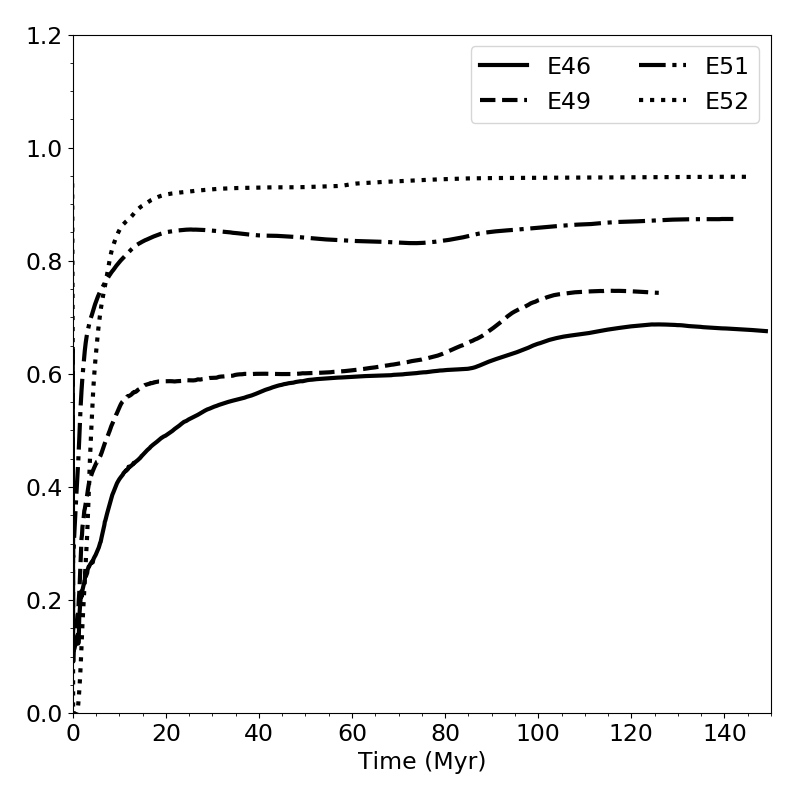
\includegraphics[width=0.45\linewidth]{figures/ch4/CGM_average_evolution}
  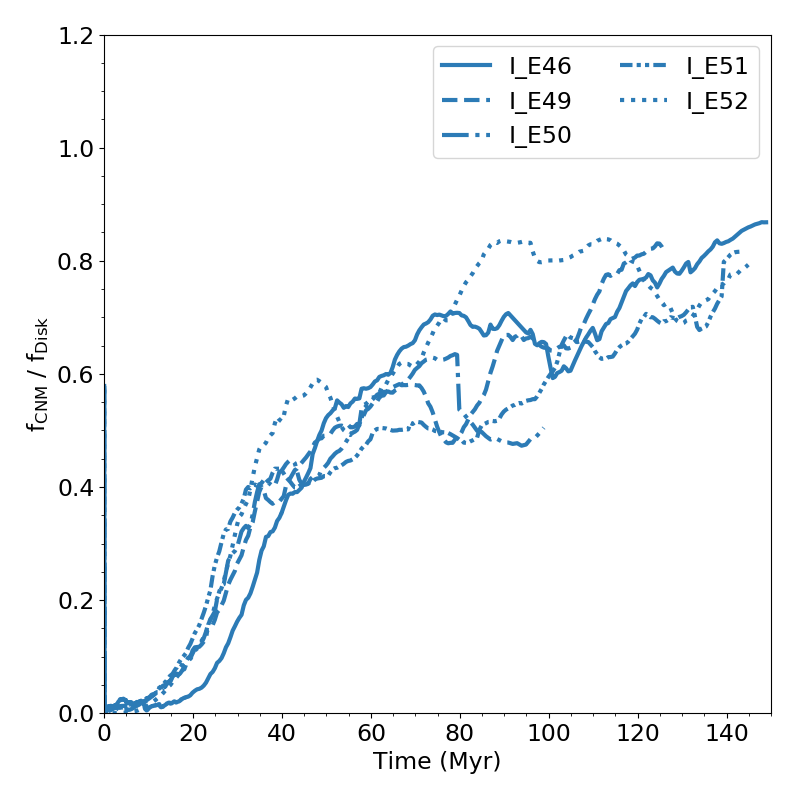
\includegraphics[width=0.45\linewidth]{figures/ch4/CNM_average_evolution}
  \caption{Time evolution of the fraction of enrichment source metals contained in the CGM over time (left), and the fraction of metals in the CNM just those metals retained in the ISM for each enrichment source (right). These are the same as the lines in Figure~\ref{ch4:fig:ISM_CGM}, but the CNM lines are normalized by the black, dashed total ISM line in Figure~\ref{ch4:fig:ISM_CGM}.}
  \label{ch4:fig:CGM_CNM}
\end{figure*}
% make a figure here showing JUST the CNM evolution of the ISM for each source

However, the metals from each source do gradually trend towards a fraction of $\sim$0.8 by the end of the 150~Myr simulation time, corresponding to the mass fraction of the CNM at this point in the galaxy's evolution (see Figure~\ref{ch1:figISM_evolution}). This trend -- that the fraction of metals contained in a given phases tends towards the mass fraction of that phase -- is true across all phases in the simulation. Therefore, we can consider that the metals for each source are well-mixed across the \textit{phases} of the ISM on timescales of $\sim$100-150~Myr. This is comparable, but less than, the dynamical timescale of the galaxy, $\sim$200~Myr. These two results suggest that the delay-time between when metals are available to enrich ongoing star formation is on order of $\sim$10~Myr across sources, and only significant for the lowest (E46, AGB-like) energy sources. Although well-mixed across phases, we emphasize that this does not imply that the abundances are the same across phases nor that the metals are spatially well-mixed across the galaxy. We investigate this second point further below.

\subsection{Homogeneity of Mixing}
\label{ch4:sec:spreads}

In Chapter~\ref{ch:chapter3} we investigate the metal enrichment distributions in the ISM as characterized by the metal fraction PDFs (see Figure~\ref{ch3:fig:log-normal} and Figure~\ref{ch3:fig:phase-statistics}). We find that this PDF is generally well described as log-normal with a power law tail towards high metal fractions, and characterize its mean, median, interquartile range (IQR), interdecile range (IDR), and the difference between the mean and median (as a measure of skew) of each distribution. In general, we find that elements released in AGB-wind events are less well-mixed than elements released in SNe, as indicated by the relative size of the IQR, IDR, and mean-median difference between the two types of elements. However, these distributions arise from the contribution of many individual enrichment events across multiple sources over long periods of time. It is unclear how metals from a \textit{single} enrichment event are distributed across a galaxy over time, and how the energy associated with the event affects the homogeneity of its distribution.

To frame this analysis, lets first examine what processes affect the metal mass fraction PDF. The mean metal mass fraction for a collection of gas is simply the total metal mass divided by the total gas mass. For a collection of gas elements, the mean metal mass fraction is defined as $Z_{\rm gas} = \frac{ \Sigma Z_{\rm i}M_{\rm gas,i}}{\Sigma M_{\rm gas,i}}$, where $M_{\rm gas,i}$ is the mass of the i$^{\rm th}$ homogeneous blob of gas, and $Z_{i}$ its metal mass fraction. A completely homogeneous ISM would have a $\delta$ function metal mass fraction PDF at the mean metal fraction, or $p(Z) = \delta(Z_{\rm gas})$. By definition, then, a homogeneous distribution will have a zero-width IQR, IDR, and mean-median difference. Non-uniform enrichment in a homogeneous medium will increase each of these quantities, while mixing in a non-uniform medium will tend to decrease each. In simple models of galactic chemical evolution, the mean gas abundance -- not the median -- is followed, even though the median is more indicative of the abundance of a ``typical" gas element. Because these two quantities provide a more immediate conceptual understanding of how metals are distributed in the ISM, we focus on characterizing the inhomogeneity of the followed metals by examining the mean-median difference. Though it is necessary for this quantity to be zero for metals to be homogeneously distributed in a medium, we do note that it is not a sufficient condition (the mean of a symmetric distribution is equal to the median). However, its evolution is easy to interpret conceptually. Enrichment increases this quantity by raising the mean metal fraction while keeping the median value fixed (or only slightly increasing), so long as the newly enriched mass is a small fraction of the total gas mass (as is almost always the case). Conversely, preferential removal of metals from a medium will lower this quantity. And finally, the mixing of metal-rich gas elements with metal-poor will gradually bring the mean and median values to parity. For our numerical experiments, enrichment in the whole ISM only occurs once and ejection from the ISM is easy to follow. This allows for a more clean interpretation of the evolution than examining either the IQR or the IDR.

\begin{figure*}
  \centering
  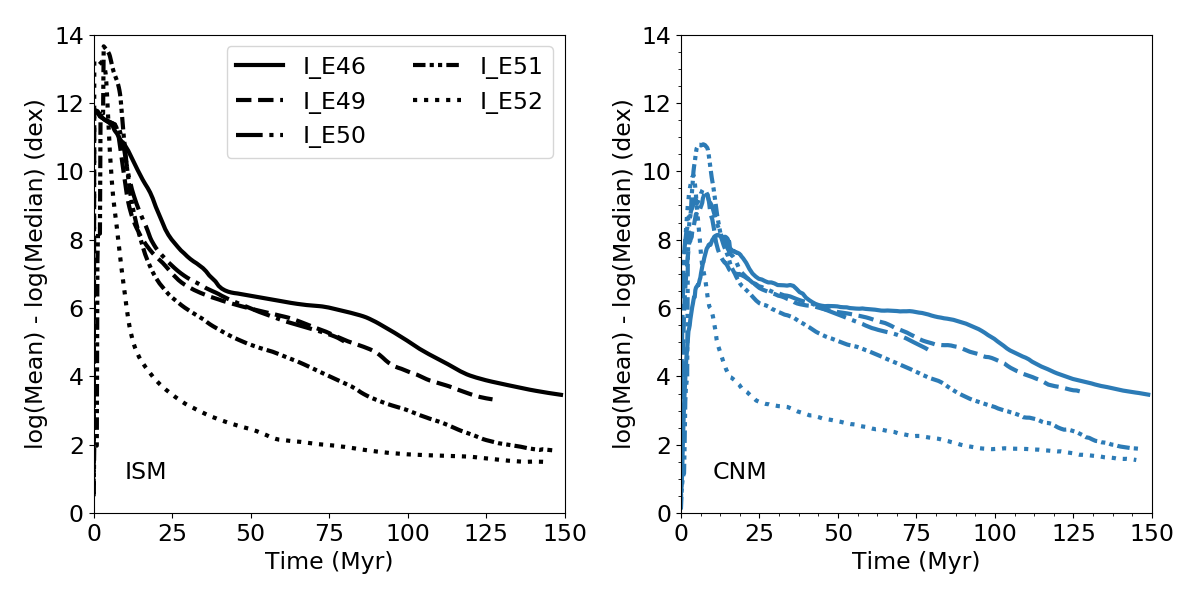
\includegraphics[width=0.975\linewidth]{figures/ch4/ISM_CNM_average_mean-median}
  \caption{Time evolution of the difference (in dex) between the mean metal mass fraction of each source and the median metal mass fraction of each source in all of the gas in the ISM (left) and in the CNM only (right).}
  \label{ch4:fig:mean-median}
\end{figure*}

In Figure~\ref{ch4:fig:mean-median} we examine the average behavior of the mean-median metal mass fractions for the whole ISM in each run (left) and the CNM only (right). In all cases, enrichment drives the dramatic increase of this value from zero to over 10 dex. This large value is due entirely because the initial abundance for each metal is near zero and thus a majority of the gas (by mass) is at an arbitrarily small metal mass fraction. This is followed by a significant decrease in spread over the first 25~Myr or so as metals are preferentially ejected from the ISM via outflows. The delay in this spike in the CNM (compared to the galaxy as a whole) is due to the different timescales over which most of the metals are incorporated into the cold gas, as shown in Figure~\ref{ch4:fig:ISM_CGM}.

Clearly, at no point can any of these distributions be considered well-mixed within the 150~Myr simulation time. \textit{Need to fix up: This is in agreement with the understanding that the mxiing timescales should correspond to XXX, which suggests that it would take $\sim$X~Gyr (1 Gyr?) for the metals to be fully mixed}. Interestingly, however, the injection energy for a given source leaves an indelible impact on the subsequent evolution of those metals in the ISM throughout the simulation time. We demonstrate that variations in abundance spread across elements may be driven significantly by the enrichment site and its associated $E_{\rm ej}$. Metals from \runone E46 are significantly less well-mixed than their higher-energy counterparts at \runone E51 and \runone E52. Interestingly, \runone E49 behaves much more similarly to \runone E46 -- with poor mixing -- even though it is much closer in energy to the \runone E51. For what mixing does occur in the CNM for these elements, it is apparent that it happens much faster ($\sim$20~Myr) for the highest energy event than the lower energy events which take longer to plateau to a consistent value.

We note that these results are given for the average behavior of \textit{single} enrichment events. If many events occur throughout the galaxy with similar metal yields then this would tend to decrease the abundance variations across the galaxy. Indeed, the recovered metal mass fraction spreads from our fiducial simulations in Chapter~\ref{ch:chapter3} are much lower ($\sim$~1- 2 dex) than the $\sim$~2-5 dex widths we find here. However, it is still true that the the AGB wind metals examined in Chapter~\ref{ch:chapter3} are more heterogeneously distributed than core collapse SNe elements in spite of the fact that these events are both more common than SNe and are more evenly distributed throughout the galaxy.

What this does suggest, however, is that in utilizing stars with unusual abundances at low metallicities to infer the yields of exotic enrichment sources, the spread of abundances in those stars may provide an important insight into the origin of those metals. For example, r-process enrichment from exotic enrichment events like hypernovae should manifest itself as more well-mixed than if the elements originated in lower energy NS-NS mergers. Conducting this analysis requires measured r-process abundances for a large sample of stars in an individual dwarf galaxy. This is challenging for the lowest mass, most metal poor dwarf galaxies, which typically only have a few to 10 stars with measured abundances, but could be done for more a few low mass dwarfs like Ursa Minor, and for more massive dwarfs like Carina, and Fornax \citep{Suda2017}.
% somerthing about needing cool onezone chemical models to try and model data with many free params might be nice here.


\subsection{Event-by-Event Variation}
\label{ch4:sec:individual event variation}

For clarity we have focused on the \textit{mean} evolution of individual enrichment events at fixed injection energy in the results thus far. We turn now to discuss how much variety exists among these individual events. For each of the discussed runs (from set \runonenu), Figure~\ref{ch4:fig:CGM_CNM_variance} shows the fraction of metals ejected from the galaxy (left) and the fraction of metals in the ISM within the CNM (center) as a function of source energy at two different times, 20~Myr (blue) and 100~Myr (orange). In the right panel, we show how the spread at each of these times varies for each event. The averaged values at each energy are shown as points, and the bars denote the min/max value for each event energy.\footnote{While the standard deviation or IQR may be more informative here, rather than min / max, the sample size at each energy, with the exception of the E46 runs, is too small to reliably do so.} As shown, there is substantial variation at each energy. This is particularly striking for the E46 events, which seemingly can have any value of $f_{\rm CGM}$ and $f_{\rm CNM} / f_{\rm Disk}$ at any point during the evolution. Finally, the right panel shows that the degree of inhomogeneous mixing for each event varies significantly as well. However, there is a more clear trend for each of the mean, min, and max values of the spread at 100~Myr (decreasing as a function of increasing $E_{\rm ej}$).

 \begin{figure*}
   \centering
   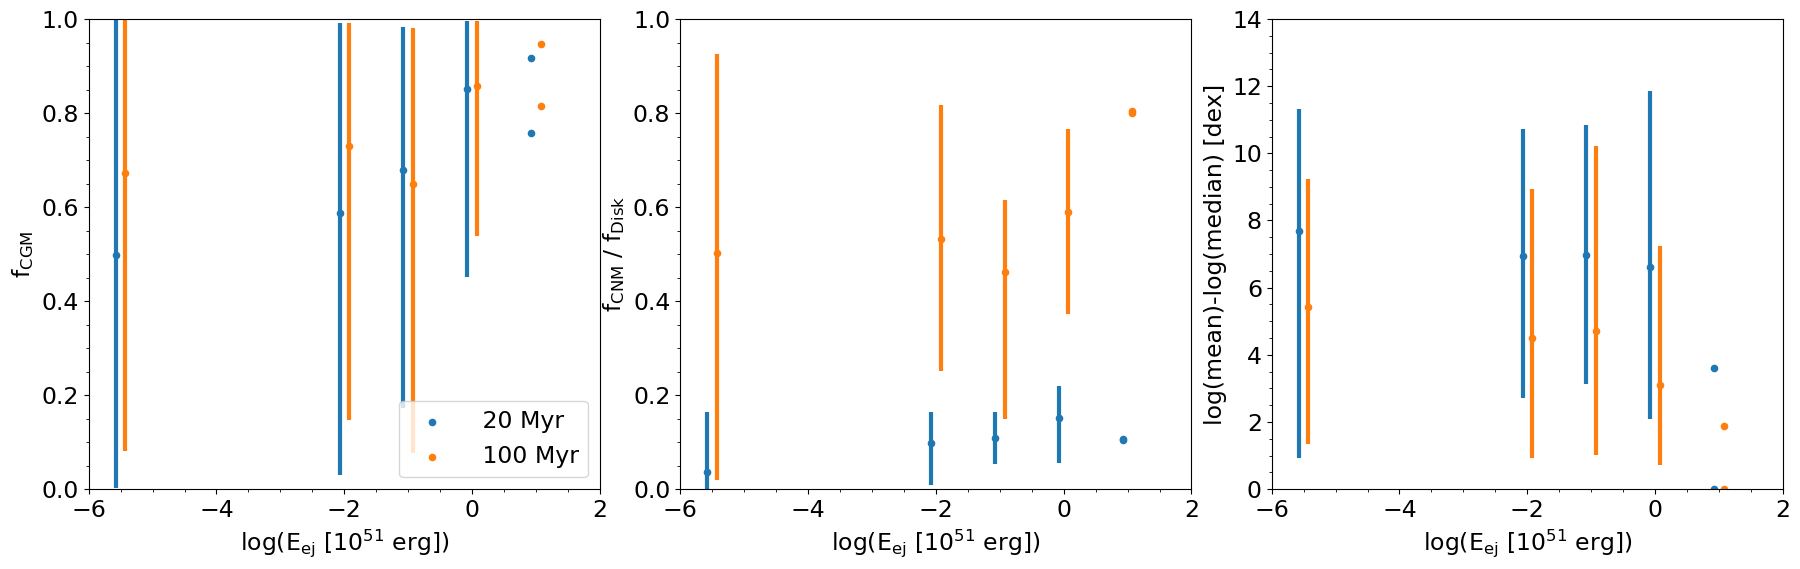
\includegraphics[width=0.975\linewidth]{figures/ch4/II_Eej_CNM_avg}
   \caption{A summary of the results presented in Figure~\ref{ch4:fig:CGM_CNM} and Figure~\ref{ch4:fig:CGM_CNM} that demonstrates the significant variation in $f_{\rm CGM}$, $f_{\rm CNM} / f_{\rm Disk}$, and the mean-median separate at fixed injection energy. The points give the average values at each energy at two different times, while the error bars show the min/max values at each energy. The points at different times have been offset slightly along the horizontal axes for clarity. Since they are only two points, we show the results from \runone E52\_r0 and \runone E52\_r300 without averaging.}
   \label{ch4:fig:CGM_CNM_variance}
 \end{figure*}


It is clear that the trends discussed thus far applies to the average behavior of events at a fixed $E_{\rm ej}$, but not for an individual event. In addition, a higher $E_{\rm ej}$ seems to increase the minimum $f_{\rm CGM}$ and $f_{\rm CNM} / f_{\rm Disk}$ expected, but the behavior of any one event must depend on additional factors. But what causes this variation among individual events? Do additional properties about the injection site (ISM density, position, local SFR), determine the subsequent evolution? Or is this the result of a non-deterministic set of complex interactions the metals from a given event experience over their lifetime in the galaxy? We investigate the dependence on a few of these properties below.

\subsection{Dependence on Radial Position}
\label{ch4:sec:radial position}
We place each source at regular, but arbitrary, positions in the galaxy without consideration for the local ISM conditions at injection. Sources are placed at the center of the galaxy ($r = 0$~pc) or at various radii (at cardinal positions at 300~pc, and 600~pc), all in the mid-place of the galaxy. Since the E46 events were likely to not self-interact, we additionally placed events at $r = 100$~pc and one event at each $r$ at about one scale height above the disk ($z = 50$~pc). For each \runonenu~ run, we plot $f_{\rm CGM}$ and $f_{\rm CNM} / f_{\rm Disk}$ as a function of radial position in the galaxy for each event in Figure~\ref{ch4:fig:radial position}. The points, error bars, and colors are the same as in Figure~\ref{ch4:fig:CGM_CNM_variance}.

 \begin{figure*}
   \centering
   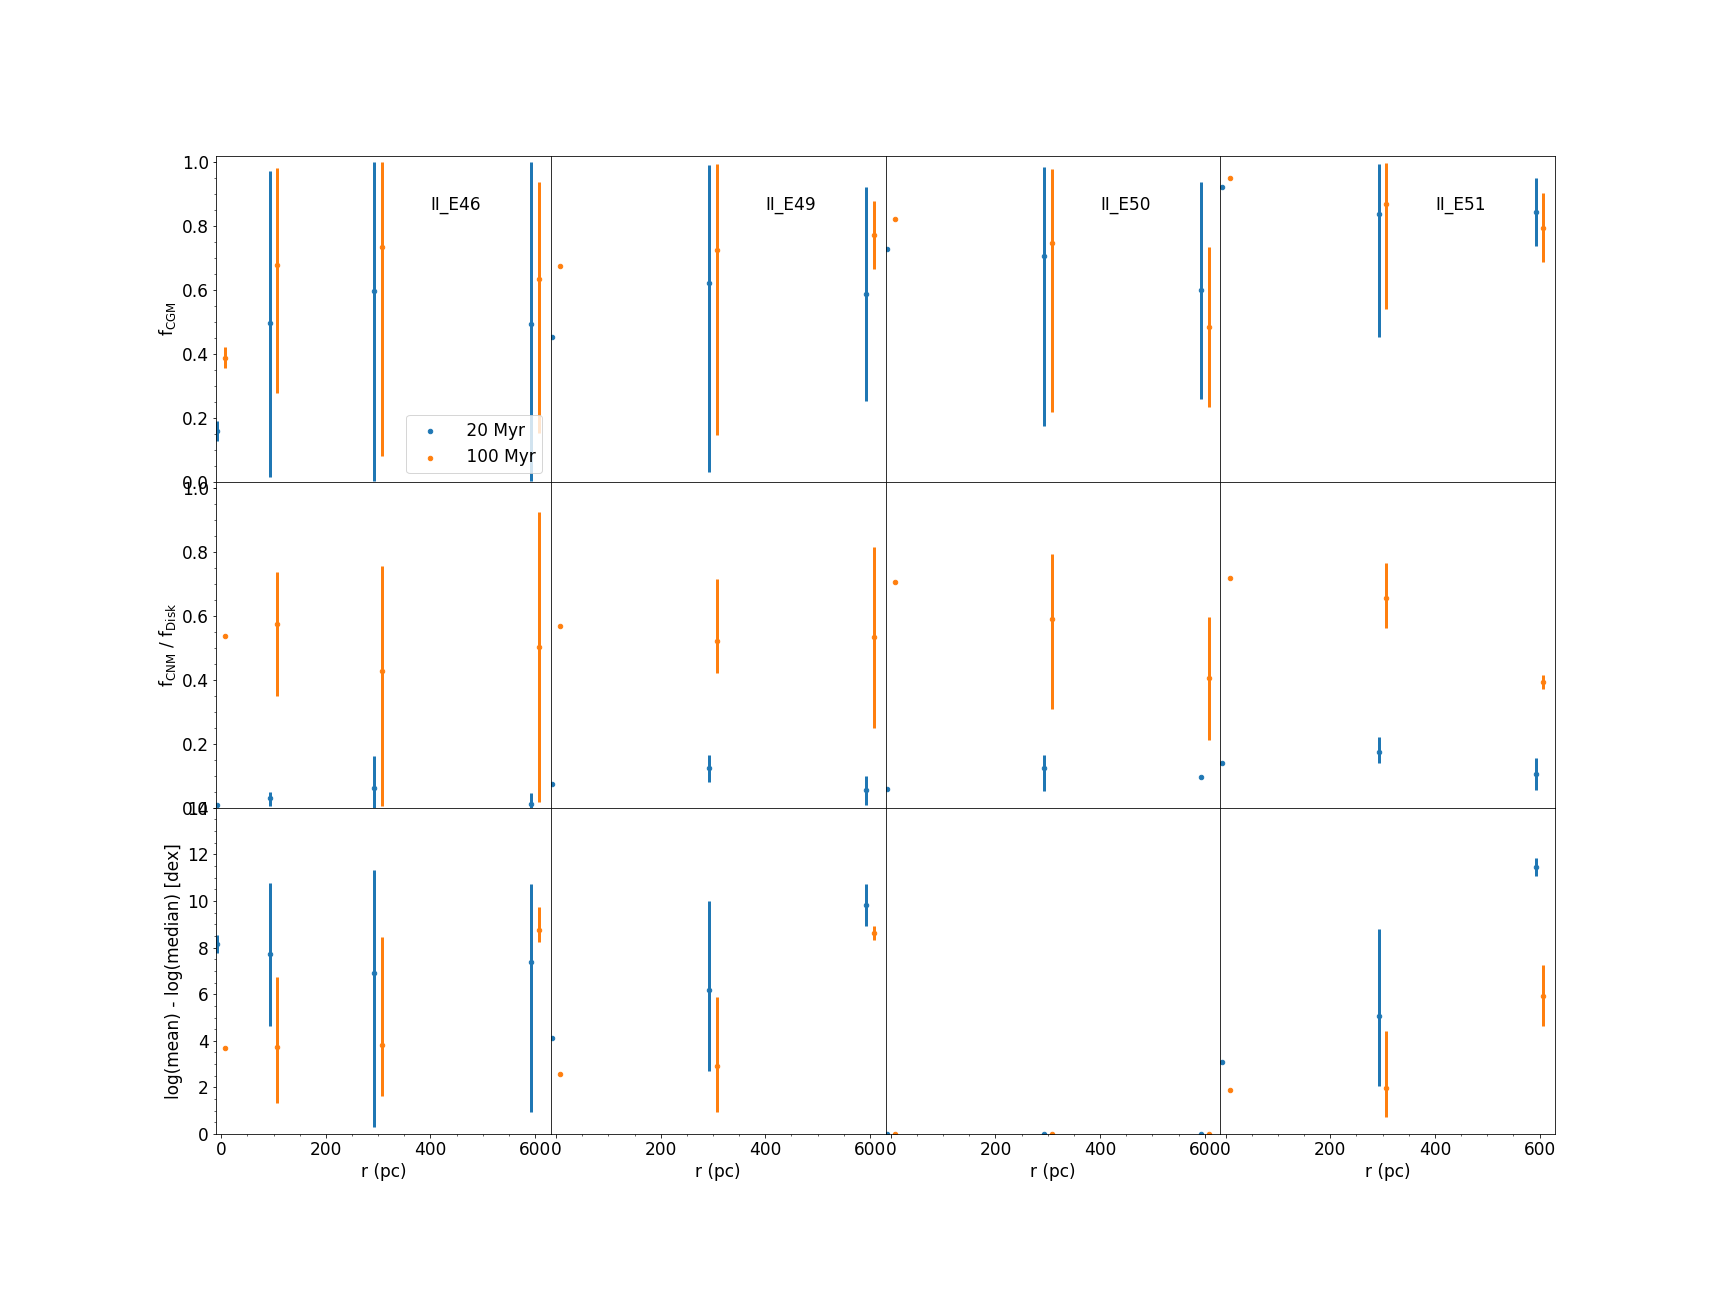
\includegraphics[angle=90,width=0.99\linewidth]{figures/ch4/II_radial_dependence}
   \caption{The dependence of $f_{\rm CGM}$ and $f_{\rm CNM} / f_{\rm Disk}$ on the radial position of each event at two different times in the evolution of the galaxy. The meaning of each point, the error bars, and colors are the same as in Figure~\ref{ch4:fig:CGM_CNM_variance}.}
   \label{ch4:fig:radial position}
 \end{figure*}

Across runs, there is no clear dependence on the radial position of the event and the fraction of metals ejected beyond the galaxy for any of the displayed runs at either 20~Myr or 100~Myr. There is a slight increase in the minimum fraction of metals ejected from the galaxy as a function of radius for the higher energy runs ($>10^{50}$~erg). This is perhaps not surprising for the largest radii as 600~pc is right near the very edge of the galaxy's disk. But again, the trend is weak and there is clearly still a great variance at both fixed $E_{\rm ej}$ and $r$. The fraction of metals in the ISM that are contained within the CNM (middle row) do not show any obvious trend at E46, but does seem to generally be lowest for the higher energy sources at the outskirts of the galaxy. Finally, the radial position does seem to affect the mixing behavior. Sources at the outskirts of the galaxy tend to be more inhomogeneous than sources at inner radii, especially at 20~Myr for the higher energy events, and the variation in behavior for these sources decreases substantially, particularly at 100~Myr. It is unclear what exactly drives these mixing differences. If feedback-driven turbulence is the dominate driver of ISM mixing in this dwarf galaxy -- as it likely is -- then sources near the center are more likely to be affected by more feedback events (due to a slightly higher $\Sigma_{\rm SFR}$) and mix more efficiently.

\subsection{Variation with Local ISM Conditions}
\label{ch4:sec:ISM density}

We compute the average ISM properties within a 4-zone radius ($4 \times dx$~=~7.2~pc) around each injection site to examine any potential correlations in evolution with ISM properties.\footnote{Note that the injection region for each event is a 3-cell radius sphere mapped onto the grid with a CIC interpolation scheme.} In Figure~\ref{ch4:fig:ISM_variance} we plot $f_{\rm CGM}$ and $f_{\rm CNM} / f_{\rm Disk}$ for each \runonenu~ run as a function of the average number density ($<n>$) in the injection region within 0.1~Myr (our time resolution) of the event. The E46 events clearly do a better job sampling the ISM density PDF, with a slight trend of decreasing $f_{\rm CGM}$ (more retained metals) with local ISM number density. This difference is even true after 100~Myr of evolution, but still with significant variation at fixed $n$. The number statistics limit a conclusive result for the higher energy events, but generally there does not appear to be an obvious trend in behavior of $f_{\rm CGM}$ as a function of $n$. This is perhaps because these energies are sufficient to heat up and dramatically reduce the density of the ISM in the injection region regardless of $n$. This is not the case for the E46 events. $f_{\rm CNM} / f_{\rm Disk}$ does not display any significant variation with $n$ at 100~Myr, but is slightly elevated at 20~Myr at higher densities. There is still a variety of behavior at fixed $n$. Finally, we note no obvious trends of the spread of the metal PDFs as a function of $n$ for all but the E46 run. Again, the local ISM densities is likely not too dynamically relevant to the higher energy events -- hence their lack of variation with $n$ -- but this is not true for E46. There is a fairly clear trend of increasing inhomogeneity in the CNM as a function of the initial $n$ in the injection region for E46, that is not present at 20~Myr, but is obvious at 100~Myr.

 \begin{figure*}
   \centering
   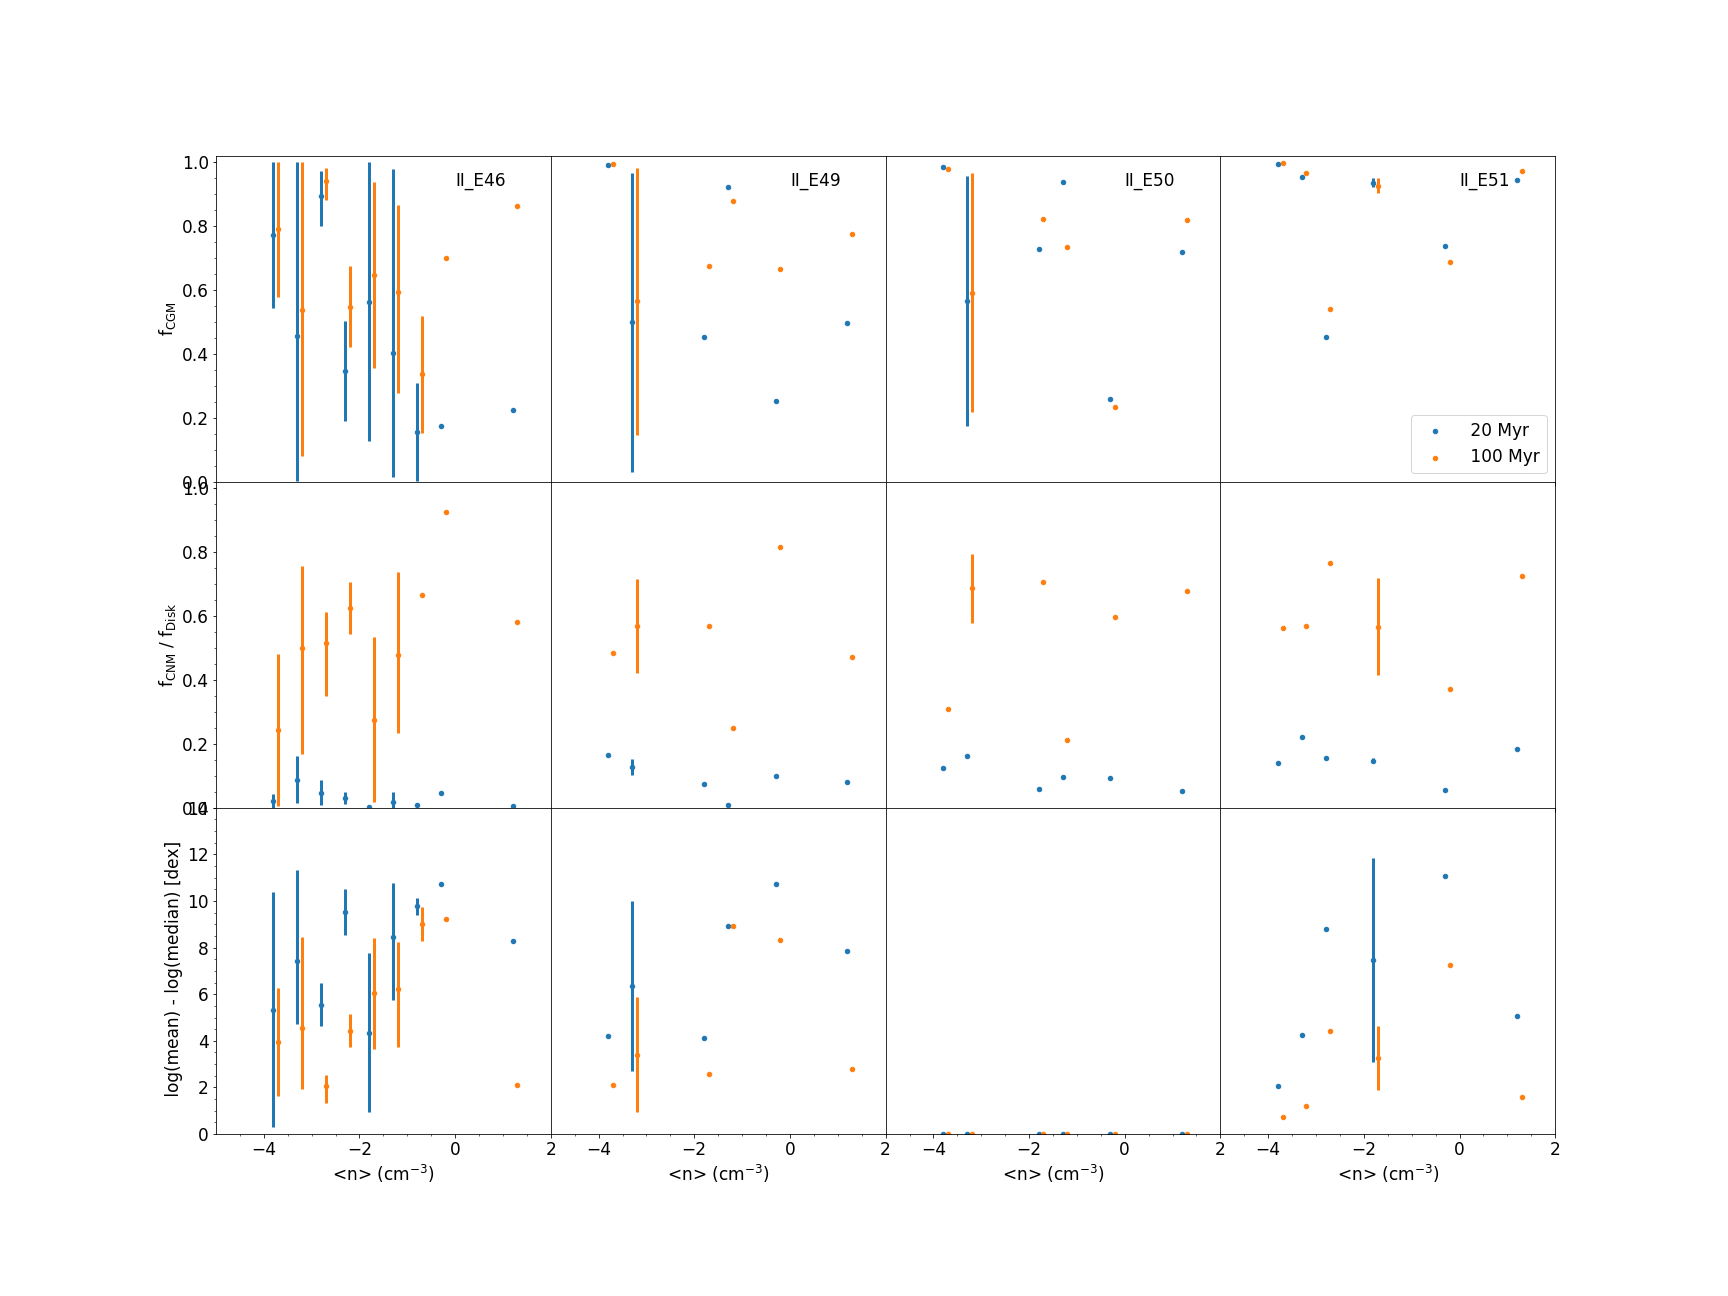
\includegraphics[angle=90,width=0.99\linewidth]{figures/ch4/II_n_dependence}
   \caption{The variation of $f_{\rm CGM}$, $f_{\rm CNM} / f_{\rm Disk}$, and the spread of the metal fraction PDFs in the ISM as a function of the local ISM number density ($n$) within the injection region of the event just prior (within 0.1~Myr) of the event. Points, lines, and line colors mean the same as shown in Figure~\ref{ch4:fig:CGM_CNM_variance}}
   \label{ch4:fig:ISM_variance}
 \end{figure*}


\subsubsection{Variation with SFR}
\label{ch4:sec:SFR}

Finally, we examine the companion run (\runtwonu) to see if the global star formation rate of the galaxy drives variation in these results. Although this does not help to directly account for the variation seen in the previous plots, this could provide insight into how SFR (in an averaged sense) affects the evolution of metals. We note that correlation with SFR is of interest not because the formation of stars by themselves, but rather the increase in feedback associated with a higher SFR (and thus a warmer / hotter ISM, greater turbulence in the ISM, and more significant outflows). We compare these two runs in Figure~\ref{ch4:fig:SFR_comparison_CGM_CNM}, showing runs from \runonenu~ in green and runs at the lower SFR, \runtwonu, in purple. $f_{\rm CGM}$ increases much more rapidly across injection energies in \runonenu. However, this value seems to be similar across runs for E49 and E51 by $\sim$50 Myr, with an additional increase again in the \runonenu~ simulations towards the end of the time. This initial spike, lull, and second increase corresponds to the period of active star formation, slightly lull, and increase in SFR experienced during the \runonenu~ simulations (see Figure~\ref{ch1:figsfr_mass_evolution}; the lull occurs between 40 and 80 Myr after the enrichment events, or during 220 - 260 Myr in that figure). The SFR is consistently low (or zero) throughout \runtwonu, with just a couple brief increases in SFR. Although E49 and E51 exhibit similar behavior across global differences in SFR, the difference in E46 is significant throughout the examined time period. As these sources do not contain enough energy to eject their metals from the galaxy by themselves, they are only ejected from the galaxy by being swept up in the ISM during other feedback events. The evolution of these events are therefore much more dependent upon the global galaxy properties.

The fraction of metals contained within the CNM of the ISM does not seem to depend too strongly on the SFR, unlike $f_{\rm CGM}$. It is generally true that after the initial $\sim$50 Myr of enrichment, a greater fraction of the metals in the ISM are contained in the CNM during the run with the lower SFR (\runtwonu), but this difference is not large and is only significant for the higher energy events. In addition, the mass fraction of the CNM is greater during run \runtwonu~ than in run \runonenu, so it may simply be that the long-term evolution of the fraction of metals in the CNM is more dependent upon the phase structure of the ISM -- which is regulated by stellar feedback -- than the feedback directly.

\begin{figure*}
  \centering
  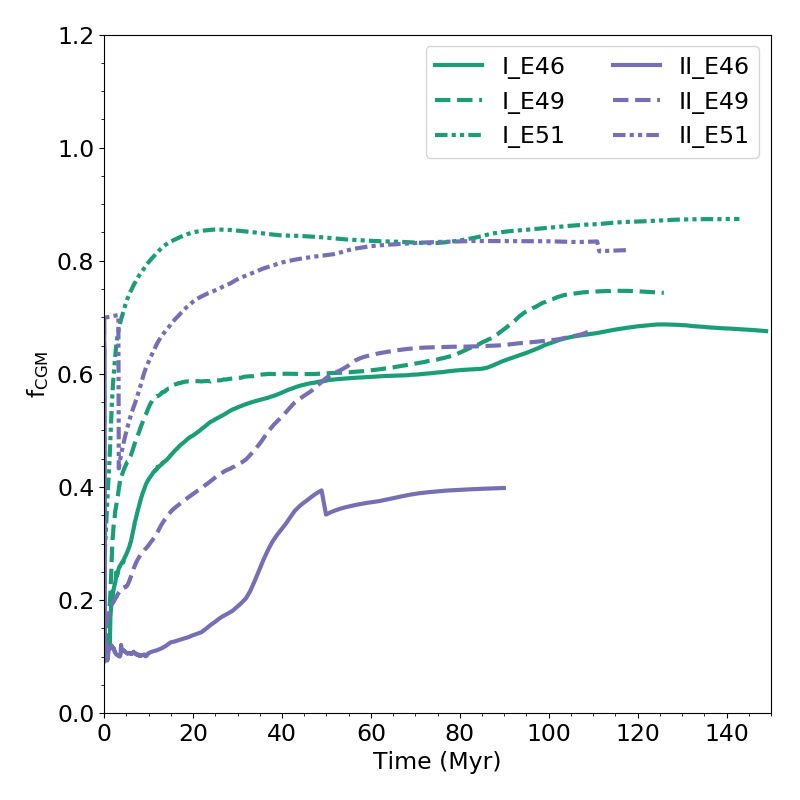
\includegraphics[width=0.45\linewidth]{figures/ch4/combined_CGM_average_evolution}
  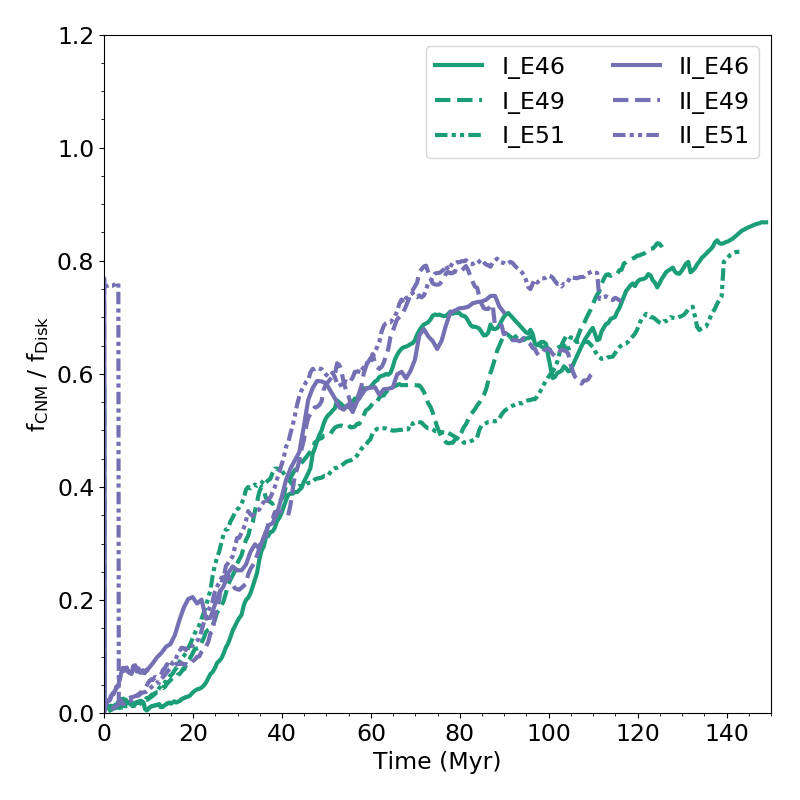
\includegraphics[width=0.45\linewidth]{figures/ch4/combined_CNM_average_evolution}\\
  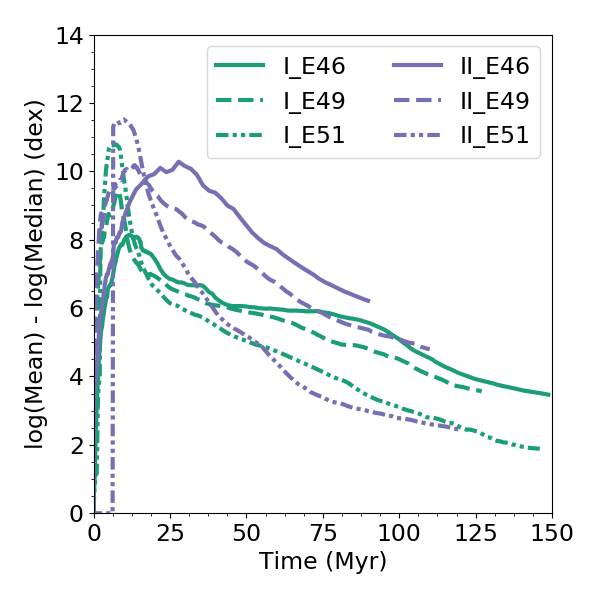
\includegraphics[width=0.45\linewidth]{figures/ch4/combined_CNM_average_mean-median}
  \caption{The same as Figure~\ref{ch4:fig:CGM_CNM}, but comparing across both sets of runs with different SFRs. Comparing across line colors for a fixed linestyle compares the difference the global SFR has on the average enrichment evolution for both $f_{\rm CGM}$ and $f_{\rm CNM} / f_{\rm Disk}$.}
  \label{ch4:fig:SFR_comparison_CGM_CNM}
\end{figure*}

Finally, examining the last panel of Figure~\ref{ch4:fig:SFR_comparison_CGM_CNM}, it does appear that the mixing efficiency of metals for each source increases with increasing global SFR. In the initial evolution, all events in run \runtwonu exhibit larger abundance spreads that take longer to begin mixing substantially than their counterparts in \runonenu. In general, \runtwonu~abundances remains larger for the first 100~Myr. The differences depend on the ejection energy, with the most significant difference found in comparing the E46 runs.
% May need more text here

\section{Discussion and Conclusions}
\label{ch4:sec:discussion conclusion}

Galactic chemical evolution is far from ``one-zone" and metal mixing is clearly neither homogeneous nor instantaneous. As demonstrated in our simulations published as \cite{Emerick2018b} and as found in the analytic work of \cite{KrumholzTing2018}, the properties of metal mixing in the ISM of various galaxies depends upon the characteristics of the individual sources -- namely the energy with which they eject metals into the ISM. This sets the thermal phase in which these metals couple to most effectively, and the volume over which they are initial injected before additional mixing by global galactic dynamics begins to dominate. In short, lower energy enrichment events, like those from AGB winds, mix much more slowly throughout the ISM than metals from higher energy events, like supernovae. As found in \cite{Emerick2018b}, this difference is still present even when accounting for the fact that AGB events are both more common and evenly distributed in the galaxy than SNe. In the new work discussed in this chapter, we further explore this behavior to try and determine the evolution of individual enrichment sources -- rather than just the average behavior of many sources -- and to explore how $E_{\rm ej}$, radial position in the galaxy, local ISM density, and global galaxy SFR affects the evolution of these metals.

We confirm the average trends found in previous works that sources with lower $E_{\rm ej}$ have larger abundance spreads in the ISM and lower ejection fractions, on average. In addition, we find that $E_{\rm ej}$ of the event and the global SFR during the time at which the event occurs produce the greatest variation in how many metals are retained by the galaxy, what fraction of those metals are contained within the CNM, and their homogeneity. Metals are in general ejected more effectively and mix more efficiently during periods of higher SFR than low, corresponding to periods of more effective galactic outflows and greater turbulence in the ISM. Although we have limited statistics to determine a conclusive trend, we generally find that the radial position at which the event occurs and the local ISM density in which the event occurs to not have a significant effect on the average behavior of enrichment events, with the exception of the lower energy (E46) events. However, we find these results to only be loose trends about the average behavior of enrichment sources. The evolution of individual events can be dramatically different, even at fixed energy and global galaxy SFR.

Variations with individual events in the above results suggests that it would be challenging to make any conclusive statements about the enrichment behavior of single enrichment sources. \textbf{Go back and look again at one-shot enrichment paper} This is problematic for interpreting the chemical abundances in UFDs that are likely to have been host to just a single, exotic enrichment event. Using these observations to constrain the total nucleosynthetic yields of these sources requires implicit assumptions about how quickly metals are available in star forming gas, how homogeneously they are distributed throughout the galaxy, and what fraction are ejected from the galaxy. It is likely that none of these quantities can be determined as simple parameters based upon the feedback properties of a single enrichment source or even the global properties of a galaxy (such as $M_{\rm halo}$, $\Sigma_{\rm SFR}$, $\Sigma_{\rm gas}$). However, this study has shown that these parameters can be characterized in an averaged sense, even though the exact result is subject to substantial stochastic effects. This, combined with some mechanism to provide this stochasticity, can be used in combination with many runs of a simple galactic chemical evolution model to understand the possible outcomes for various galaxies. Developing such a model will be a powerful tool for interpreting the irregular stellar abundance patterns observed in low mass dwarf galaxies in the nearby Universe.


%************* APPENDICES ************************%

%\section*{Acknowledgments}

%\clearpage
%\appendix - Liklely DO NOT use this command
\setcounter{section}{0}%
\renewcommand\thesection{\thechapter.\Alph{section}}

%
% Place appendix here
%

\renewcommand\thesection{\thechapter.\arabic{section}}
